\documentclass[9pt,twoside,lineno]{pnas-new}
% Use the lineno option to display guide line numbers if required.
\usepackage{subcaption}
\usepackage[figuresleft]{rotating}
\usepackage{fixme}

\templatetype{pnassupportinginfo}
%\readytosubmit %% Uncomment this line before submitting, so that the instruction page is removed.

\title{The Wisdom and Manipulability of Threads}
\author{Robin Engelhardt, Jacob Stærk-Østergaard, Vincent F. Hendricks}
\correspondingauthor{E-mail: robin@hum.ku.dk}

\begin{document}

%% Comment/remove this line before generating final copy for submission
%\instructionspage  

\maketitle

%% Adds the main heading for the SI text. Comment out this line if you do not have any supporting information text.
\SItext

\subsection*{Data Collection}
Controlled lab experiments of thread dynamics are rare in the research literature due to the difficulties in keeping a large number of participants in a queue. We designed our experiment along the same lines as the classical information cascade laboratory experiments by Anderson and Holt  that were created to understand student's decision-making behavior in in a sequential decision structure where it can become sensible to ignore private signals due to the aggregation of public knowledge about preceding decisions \cite{anderson1997information}. While such a design is not very feasible in normal laboratory conditions (at least for threads with several hundred participants), it is well suited for online labor markets and crowdsourcing platforms such as Amazon Mechanical Turk (Mturk), an online labor markets and crowdsourcing platform that has become a highly valued tools for social scientists who wish to conduct experimental research on the real time dynamics of large groups. Mturk has repeatedly been shown to meet or exceed the standards set by data collection methods using other means \cite{berinsky2012evaluating, buhrmester2018evaluation}. The platform provides an integrated participant compensation system, has a large participant pool, and has been shown to be reliable, replicable, and significantly more diverse than typical American college samples \cite{mason2009financial, buhrmester2011amazon, crump2013evaluating, rand2012promise, horton2011online}.

\subsection*{Experimental Setup}
Our experimental setup on Mturk is simple. After accepting our ‘HIT’ (Mturk acronym for a ‘human intelligence task’) and providing informed consent, participants are asked to wait in a ‘waiting room’ until the ‘choice room’ (through which all participants have to go sequentially) becomes available. After entering the choice room, participants are asked to take a look at the image and make an estimate (see screenshots in figures S1 and S2).

Depending on the view condition, participants can see $v\in\{0,1,3,9\}$ preceding estimates. We chose to present the ‘oldest’ previous estimate on the top of the list and the last estimate made on the bottom. When dealing with news, or financial data, users typically want to see the most recent activity first (think tweets, online banking transactions, news updates). With conversations it is different because there is a context to consider of whatever message came before and after the one you are looking at (think blogs or facebook comments). We have chosen to use the conversation thread design (oldest on top) because there is no particular news criteria when guessing the weight of an ox or estimating the number of dots on a screen.

Participants have one minute to think about the image and make their estimate. This might sound as a severe time constraint, but exploratory trials have shown that participants in general use less than a minute when performing this task. Since participants come from all over the world, they can submit their estimate in units of kilo or in units of pounds. After submission, participants are thanked for their participation and the experiment ends. Waiting times are compensated with \$0.20 per minute (maximally 5 minutes), participation fee is \$0.10, and a bonus of \$1 is paid if an estimate is within 10\% of the true weight of the ox.

\subsection*{Mturk Settings}
When working with Mturk it is important to consider the right settings in order to get the best data quality possible \cite{chandler2016conducting}. Fair wage, attrition rates, removal of duplicate participants and informative feedback are some of the most important issues to address.

Average wage for participants in our experiments was $\sim$ \$12 per hour, which is considered good according to Mturk guidelines and certainly above the estimated average of \$6 per hour when excluding un-submitted and rejected work \cite{hara2018data}.

Quitting a study before completing it is prevalent on Mturk, and varies systemically across experimental conditions \cite{zhou2016pitfall}. For the ox-experiments attrition rates were between 20-40\% due to an unanticipated large amount of participants accepting the HIT in the first few minutes. On average 20 participants accepted our HITs within the first minute; after 10 minutes the average acceptance rate had dropped to 2-3 participants per minute and after an hour to less than one participant per minute. Our scripts were coded in such a way that participants were automatically assigned to a ‘waiting room’ in which they were asked to wait for maximally five minutes before entering the choice room. This meant that a lot of participants waited in vain. Due to such a high attrition rate in the first couple of experiments we changed the script slightly later on: Now the waiting room could contain a maximum of five participants, and when the waiting room was full, participants were told to come back and finish the HIT at a later point in time. This reduced the attrition rate to 10.5\% on average.

All participants automatically received an image-specific qualification when accepting a HIT. This qualification ensured that participants could not accept any other HITs that use the same image. Further data inspection showed that 33 participants somehow managed to accept two HITs with the same image anyway. The reason may be that the time interval between accepting two HITs with the same image was too short for the qualification to register in the Mturk interface. All 33 duplicate participants were removed before data analysis. In addition, we set the qualification that participants should have completed at least 100 HITs and have an accepted HIT rate of 98\% or above. This ensured that we would get only experienced and qualified participants.

Mturk participant attention was expected to be equal to or better than undergraduate participant’s attention \cite{hauser2016attentive}, while various forms of dishonesty (practical joking or telling others about the true value offline or on an Mturk participants web page) was expected to be rare. Our screening of data files before data analyses revealed that a small fraction of participants submitted ridiculously high estimates across images seen, thereby skewing thread averages substantially. These estimates were not treated differently, however, because we had no reason to conclude that they were made with bad intent.

During our experiments, participants had easy access to our email for questions and possible bug reports. Apart from some minor difficulties when typing from a mobile device (less than 1\%) participants had few comments or complaints.

\subsection*{Code and Software}
All experiments are coded in the experimental software otree 2.1 \cite{chen2016otree} which is based on python and django. The code itself is designed along the same lines as the classical information cascade experiments by Anderson and Holt \cite{anderson1997information}. The main feature of any cascade game is that decisions are taken sequentially. A player makes an estimate, and the next one receives the information about the estimate of the previous player (or all or some previous players). Thus, the main technical issue is that only one person at a time can make a decision while others wait. As soon as a player finishes and leaves the choice page, the next player enters while all subsequent players still have to wait. Scripts for the analysis of data and for the plotting of all figures in the main text as well as in the Supplementary Information are available on \href{https://github.com/gavstrik/WoT}{github}.

\subsection*{Data Collection}
We obtained a total of 11748 estimates from 6169 unique participants. Any dot-image was only seen once by a participant, i.e. we had a total of 3157 participants seeing only one image, 1259 participants seeing two images, 1047 participants seeing three images, and 733 participants seeing all four images (either in the unmanipulated or manipulated conditions and with $v\in\{0,1,3,9\}$). A few of the manipulated threads were stopped prematurely (containing less than 100 participants) because early outlier estimates turned the social information available to the succeeding participants into unbelievably high numbers. In those threads, the transition period from compromizing to not at all believing the social information became very short, making the thread dynamics relative uninteresting. Instead of running a highly manipulated thread for a long time, we opted for restarting the thread with new participants. See table \ref{table:S1} for a full list of threads and their summary statistics. 

\subsection*{Outliers}
Previous work has shown that distributions of independent estimates are approximately log-normal. Consequently, the arithmetic mean is usually much larger than most estimates and often larger than the true value. Testing our data we find distributions to be only approximately log-normal (see QQ-plots in figure S3 for examples). In addition, table \ref{table:S1} shows highly variable distributions of estimates. Skewnesses and kurtoses, describing the lack of symmetry and the size of the tail of the distributions, span values from close to zero to above 100. These asymmetries are reflected by the presence of outliers. 

For all reported aggregate measures, outliers are removed if they have an error rate above 10, so that $|x_r-truth|/truth <10$, where $x_r$ is the estimate by participant $r$. We also use a lower bound of $truth/10$, due some reports of not being able to see the form input on mobile devices or unanticipated timeouts (see SI Appendix, section “Mturk Settings”). With these trimming criteria in place, we count a the following number of outliers: In the dots-experiments, 62 participants have an error rate above 100, and 118 participants have an error rate above 10, while 33 participants have made an estimate below 10\% of the true value. In the ox-experiments, one participant has an error rate above 30 and 9 participants have an error rate above 10, while 94 participants have made an estimate less than 10\% of the true value. This give a total of 151 (1.8 \%) outliers in the dots-experiments and 103 (4.1 \%) outliers in the ox-experiments, giving a grand total of 254 (2.4 \%) outliers out of 10.808 estimates.



\subsection*{Analysis of thread medians}


\subsection*{QQ plots for median analysis}
"Sed ut perspiciatis unde omnis iste natus error sit voluptatem accusantium doloremque laudantium, totam rem aperiam, eaque ipsa quae ab illo inventore veritatis et quasi architecto beatae vitae dicta sunt explicabo. Nemo enim ipsam voluptatem quia voluptas sit aspernatur aut odit aut fugit, sed quia consequuntur magni dolores eos qui ratione voluptatem sequi nesciunt. Neque porro quisquam est, qui dolorem ipsum quia dolor sit amet, consectetur, adipisci velit, sed quia non numquam eius modi tempora incidunt ut labore et dolore magnam aliquam quaerat voluptatem. Ut enim ad minima veniam, quis nostrum exercitationem ullam corporis suscipit laboriosam, nisi ut aliquid ex ea commodi consequatur? Quis autem vel eum iure reprehenderit qui in ea voluptate velit esse quam nihil molestiae consequatur, vel illum qui dolorem eum fugiat quo voluptas nulla pariatur?"




"Sed ut perspiciatis unde omnis iste natus error sit voluptatem accusantium doloremque laudantium, totam rem aperiam, eaque ipsa quae ab illo inventore veritatis et quasi architecto beatae vitae dicta sunt explicabo. Nemo enim ipsam voluptatem quia voluptas sit aspernatur aut odit aut fugit, sed quia consequuntur magni dolores eos qui ratione voluptatem sequi nesciunt. Neque porro quisquam est, qui dolorem ipsum quia dolor sit amet, consectetur, adipisci velit, sed quia non numquam eius modi tempora incidunt ut labore et dolore magnam aliquam quaerat voluptatem. Ut enim ad minima veniam, quis nostrum exercitationem ullam corporis suscipit laboriosam, nisi ut aliquid ex ea commodi consequatur? Quis autem vel eum iure reprehenderit qui in ea voluptate velit esse quam nihil molestiae consequatur, vel illum qui dolorem eum fugiat quo voluptas nulla pariatur?"

\subsection*{GMM model}
"Sed ut perspiciatis unde omnis iste natus error sit voluptatem accusantium doloremque laudantium, totam rem aperiam, eaque ipsa quae ab illo inventore veritatis et quasi architecto beatae vitae dicta sunt explicabo. Nemo enim ipsam voluptatem quia voluptas sit aspernatur aut odit aut fugit, sed quia consequuntur magni dolores eos qui ratione voluptatem sequi nesciunt. Neque porro quisquam est, qui dolorem ipsum quia dolor sit amet, consectetur, adipisci velit, sed quia non numquam eius modi tempora incidunt ut labore et dolore magnam aliquam quaerat voluptatem. Ut enim ad minima veniam, quis nostrum exercitationem ullam corporis suscipit laboriosam, nisi ut aliquid ex ea commodi consequatur? Quis autem vel eum iure reprehenderit qui in ea voluptate velit esse quam nihil molestiae consequatur, vel illum qui dolorem eum fugiat quo voluptas nulla pariatur?"



In order to cope with the heavy tails present in the data a Gaussian Mixture Model (GMM) was used to model the effects of social influence. This model class utilizes multiple states to ultimately obtain a gaussian mixture distribution for each observation. Let $X=\{1,\dots,k\}$ denote the state variable and $Y$ the observation. Then, conditional on $X=s, s=1,\dots,k$, $Y$ follows a normal distribution
\begin{align*}
	Y|(X=s)  \sim \mathcal{N} (\mu_s,\sigma^2_s), s=1,\dots,k,
\end{align*}
hence the unconditional distribution of $Y$ is obtained by integrating over $X$
\begin{align*}
	P(Y) = \sum_{s=1}^k P(X=s)P(Y|X=s).
\end{align*}
Thus, given $k$ states and using $\delta_s = P(X=s)$, $Y$ is normally distributed with parameters
\begin{align*}
	\mu &= \sum_{s=1}^k \delta_s \mu_s \\
	\sigma^2 &= \left(\sum_{s=1}^k \delta_s \sigma\right)^2 \\
\end{align*}
For the analysis of this paper, this implies that the individual observations $y_i, i=1,\dots,n$ are weighted among $k$ states. This entails that the social influence on $y_i$ is a weighted sum of $k$ $\beta_\text{info}$ values. In other words, the social influence on $y_i$ is
\begin{align*}
	\beta_{w_i}	 = \sum_{s=1}^k \delta_{i,s}\beta_{s,\text{info}},
\end{align*}
where $w_i$ refer to the weighing of $k$ $\beta$-values using individual weights $\delta_{i,s}$ for each observation.

These models can effectively deal with varying 
 



\subsection*{Jayles data}
The data from \citep{jayles2017social} is similar to the Mturk in the sense that participants are given difficult estimation tasks. However, in this case, both a pre-estimate and their estimates after given social information were recorded. In addition, some manipulation took place in the sense that "expert" estimates (precise answers) were mixed into the geometric average of the social information. The questions were constructed so it would be near impossible to know precise answers on all questions. Yet the difficulty of questions ranged from easy to very difficult, in the sense that participants had more/less intuition regarding the answer and their median answer was close to the true value or far apart, see Figure \ref{fig: Jayles question difficulty}. The models were all fitted using $k=3$ states, this presented a decent fit (not shown) as evaluated by QQ-plots, as in the case of the Mturk data. 

Questions 1, 2 were of very similar type, referring to population sizes of two major Asian cities. The results in Figure \ref{fig: Jayles question 1}-\ref{fig: Jayles question 2} reveal that the participants attitude was similar in the use of social information. Roughly a third were Keepers/Contrarians (also found in Jayles??) 10-20\% were Followers and the rest (majority group) consisted of Compromisers to some extend. Questions 8 and 10, Figures \ref{fig: Jayles question 8}-\ref{fig: Jayles question 10} where very different types, although the answer was numerically comparable to Questions 1 and 2. In the case of Figure \ref{fig: Jayles question 8}, the group medians all had a negative bias, although less so with more experts included. This indicates that participants underestimated the answer to a large extend, but also weighed social information heavily. This is evident in Figure \ref{fig: Jayles question 8} where the almost complete lack of a Keeper/Contration group indicates that participants weighed their own opinion less. Regarding Question 10, Figure \ref{fig: Jayles question 10} reveals that the upper 50\% of the $\beta_w$ distribution is comparable to the one in Figure \ref{fig: Jayles question 8} on Question 8. However, clearly a significant group of participants weighed their own opinion highly due to the clear presence of a Keeper/Contrarian group. All the questions were presented to French students, which could explain this difference among Questions 8 and 10, since Question 8 dealt with the American Congress Library where as Question 10 dealt with sales of mobile phones in France. Finally, Question 23, Figure \ref{fig: Jayles question 23}, is very different from the others in both type and numerical answer. Yet this Question seemed most difficult, according to Figure \ref{fig: Jayles question difficulty}. The Figure also shows that this question benefitted the most from the introduction of expert estimates as the severe negative group bias is mitigated strongly by these experts corrections of the social information. There are a few Keepers/Contrarians among the participants on this question, however Figure \ref{fig: Jayles question 23} shows that the estimated $\beta_w$'s of this group are very imprecise, as the confidence bounds on the distribution of $\beta_w$ is very wide in the bottom end. Contrary the Followers group displays much narrower confidence bounds indicating a good estimate of the upper 50\% of the distribution. Hence, Figure \ref{fig: Jayles question 23} also indicates that Question 23 is difficult as most of the participants weigh the social information heavily, and those few who doesn't are quite difficult to categorize as the model imply they should be put somewhere between highly Contrarians ($\beta_w<0.5$) to rather heavy Compromisers ($\beta_w\approx 0.5$).

\begin{figure}[htbp]
	\centering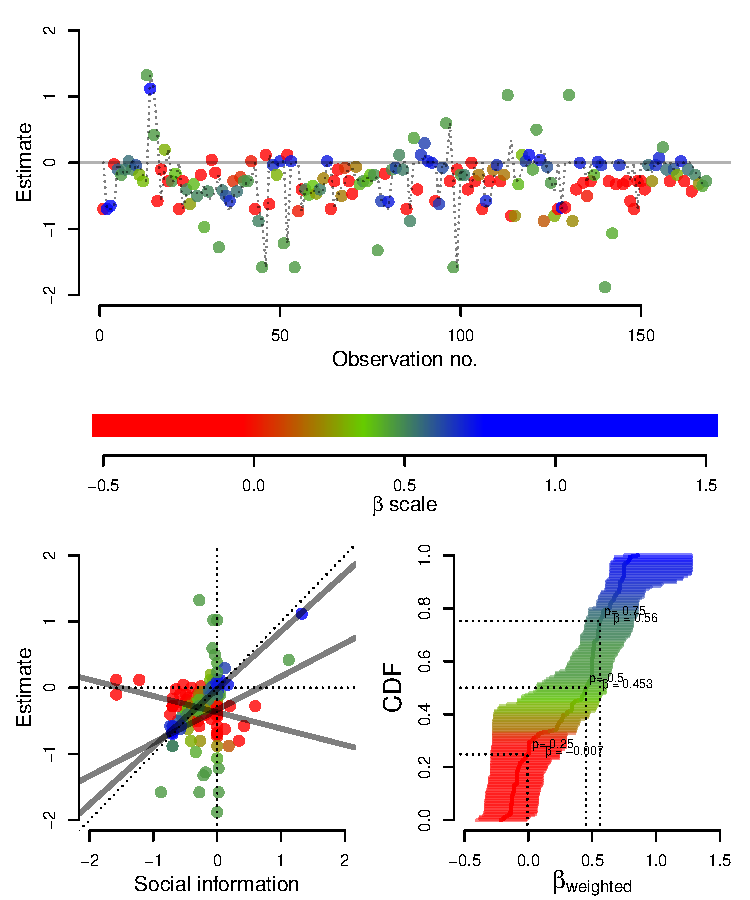
\includegraphics[width=.5\textwidth]{../plots/jayles1.pdf}
	\caption{Jayles question 1: What is the population of Tokyo and its agglomeration? True answer: 38,000,000.}\label{fig: Jayles question 1}
\end{figure}

"Sed ut perspiciatis unde omnis iste natus error sit voluptatem accusantium doloremque laudantium, totam rem aperiam, eaque ipsa quae ab illo inventore veritatis et quasi architecto beatae vitae dicta sunt explicabo. Nemo enim ipsam voluptatem quia voluptas sit aspernatur aut odit aut fugit, sed quia consequuntur magni dolores eos qui ratione voluptatem sequi nesciunt. Neque porro quisquam est, qui dolorem ipsum quia dolor sit amet, consectetur, adipisci velit, sed quia non numquam eius modi tempora incidunt ut labore et dolore magnam aliquam quaerat voluptatem. Ut enim ad minima veniam, quis nostrum exercitationem ullam corporis suscipit laboriosam, nisi ut aliquid ex ea commodi consequatur? Quis autem vel eum iure reprehenderit qui in ea voluptate velit esse quam nihil molestiae consequatur, vel illum qui dolorem eum fugiat quo voluptas nulla pariatur?"

\begin{figure}[htbp]
	\centering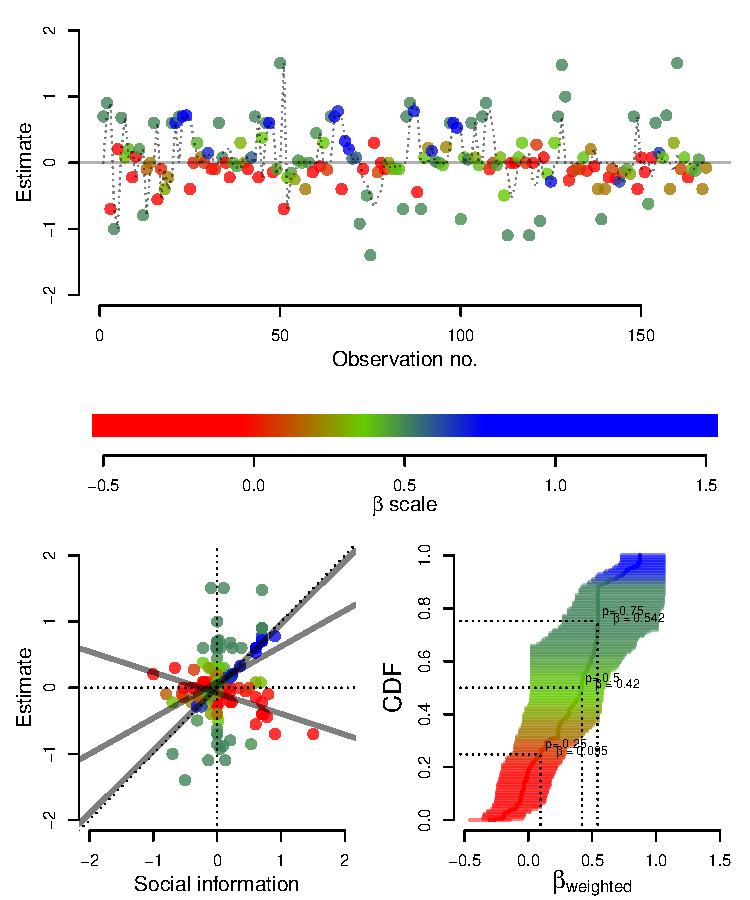
\includegraphics[width=.5\textwidth]{../plots/jayles2.pdf}
	\caption{Jayles question 2: What is the population of Shanghai and its agglomeration? True answer: 25,000,000.}\label{fig: Jayles question 2}
\end{figure}

"Sed ut perspiciatis unde omnis iste natus error sit voluptatem accusantium doloremque laudantium, totam rem aperiam, eaque ipsa quae ab illo inventore veritatis et quasi architecto beatae vitae dicta sunt explicabo. Nemo enim ipsam voluptatem quia voluptas sit aspernatur aut odit aut fugit, sed quia consequuntur magni dolores eos qui ratione voluptatem sequi nesciunt. Neque porro quisquam est, qui dolorem ipsum quia dolor sit amet, consectetur, adipisci velit, sed quia non numquam eius modi tempora incidunt ut labore et dolore magnam aliquam quaerat voluptatem. Ut enim ad minima veniam, quis nostrum exercitationem ullam corporis suscipit laboriosam, nisi ut aliquid ex ea commodi consequatur? Quis autem vel eum iure reprehenderit qui in ea voluptate velit esse quam nihil molestiae consequatur, vel illum qui dolorem eum fugiat quo voluptas nulla pariatur?"

\begin{figure}[htbp]
	\centering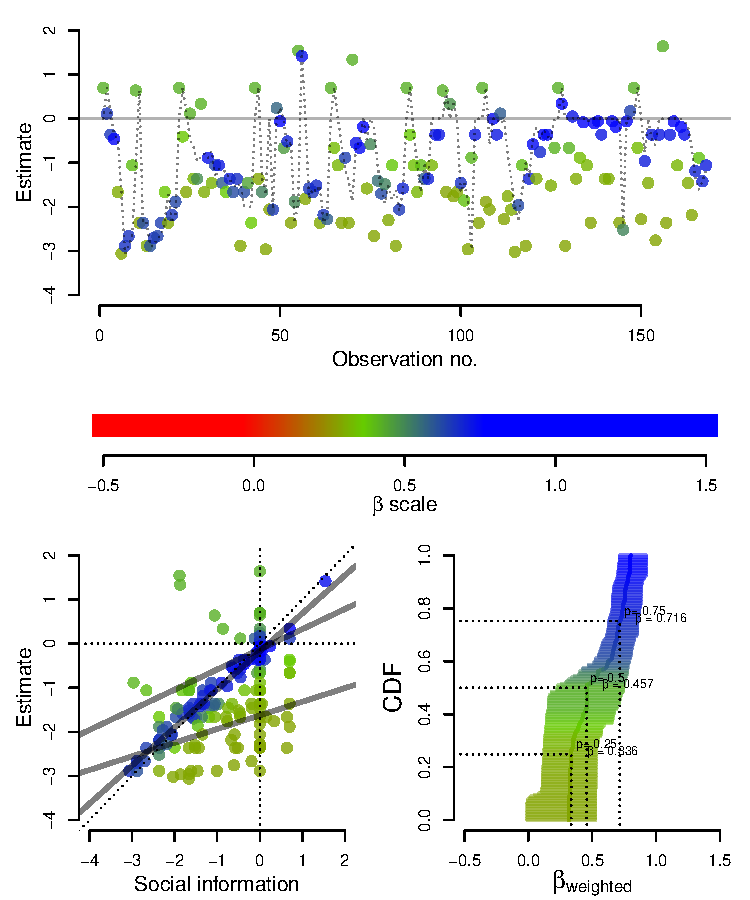
\includegraphics[width=.5\textwidth]{../plots/jayles8.pdf}
	\caption{Jayles question 8: How many books does the American Congress library hold? True answer: 23,000,000.}\label{fig: Jayles question 8}
\end{figure}

"Sed ut perspiciatis unde omnis iste natus error sit voluptatem accusantium doloremque laudantium, totam rem aperiam, eaque ipsa quae ab illo inventore veritatis et quasi architecto beatae vitae dicta sunt explicabo. Nemo enim ipsam voluptatem quia voluptas sit aspernatur aut odit aut fugit, sed quia consequuntur magni dolores eos qui ratione voluptatem sequi nesciunt. Neque porro quisquam est, qui dolorem ipsum quia dolor sit amet, consectetur, adipisci velit, sed quia non numquam eius modi tempora incidunt ut labore et dolore magnam aliquam quaerat voluptatem. Ut enim ad minima veniam, quis nostrum exercitationem ullam corporis suscipit laboriosam, nisi ut aliquid ex ea commodi consequatur? Quis autem vel eum iure reprehenderit qui in ea voluptate velit esse quam nihil molestiae consequatur, vel illum qui dolorem eum fugiat quo voluptas nulla pariatur?"

\begin{figure}[htbp]
	\centering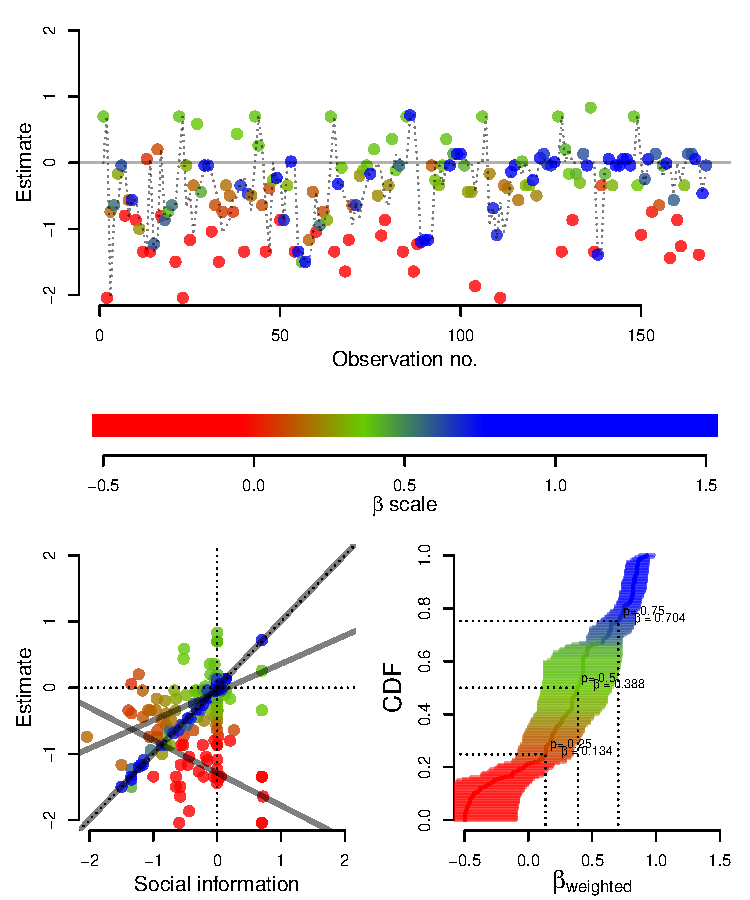
\includegraphics[width=.5\textwidth]{../plots/jayles10.pdf}
	\caption{Jayles question 10: How many cell phones are sold in France every year? True answer: 22,000,000.}\label{fig: Jayles question 10}
\end{figure}

"Sed ut perspiciatis unde omnis iste natus error sit voluptatem accusantium doloremque laudantium, totam rem aperiam, eaque ipsa quae ab illo inventore veritatis et quasi architecto beatae vitae dicta sunt explicabo. Nemo enim ipsam voluptatem quia voluptas sit aspernatur aut odit aut fugit, sed quia consequuntur magni dolores eos qui ratione voluptatem sequi nesciunt. Neque porro quisquam est, qui dolorem ipsum quia dolor sit amet, consectetur, adipisci velit, sed quia non numquam eius modi tempora incidunt ut labore et dolore magnam aliquam quaerat voluptatem. Ut enim ad minima veniam, quis nostrum exercitationem ullam corporis suscipit laboriosam, nisi ut aliquid ex ea commodi consequatur? Quis autem vel eum iure reprehenderit qui in ea voluptate velit esse quam nihil molestiae consequatur, vel illum qui dolorem eum fugiat quo voluptas nulla pariatur?"

\begin{figure}[htbp]
	\centering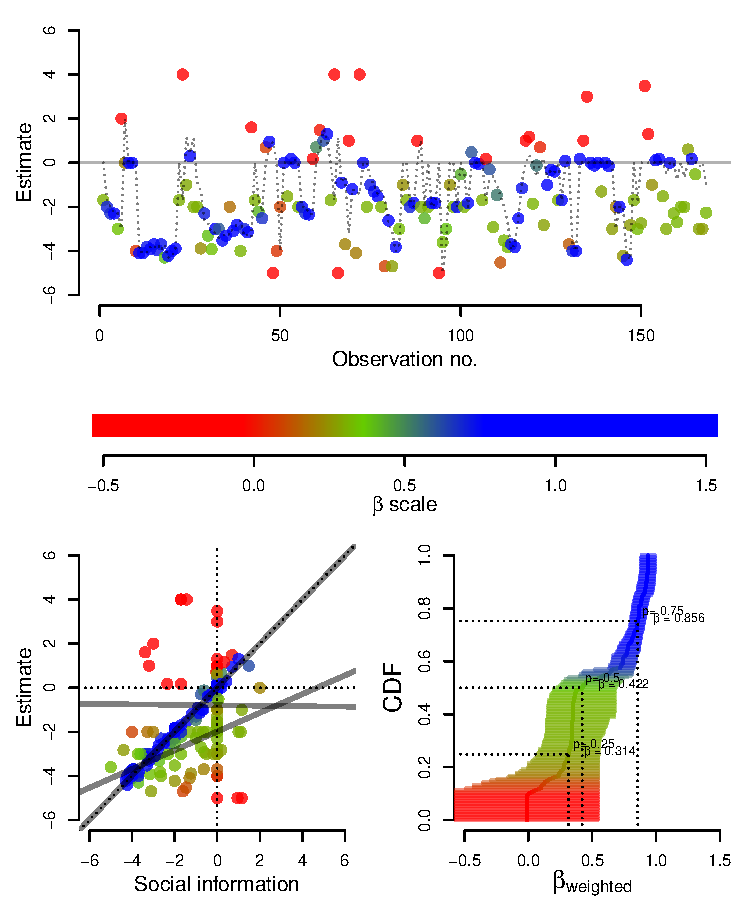
\includegraphics[width=.5\textwidth]{../plots/jayles23.pdf}
	\caption{Jayles question 23: How many galaxies does the visible universe hold (in millions of galaxies)? True Answer: 100,000.}\label{fig: Jayles question 23}
\end{figure}


\subsubsection{Jayles data, including pre-estimates}
%In order to validate conclusions on the use of social information without knowing the personal opinions, the final estimates where plottet against the pre-estimates $y_i^0$, mapping the individual colors of the $\beta_w$ scale. Hence, in Figure \ref{fig: Jayles estimate vs pre-estimate} the colors correspond to the $\beta_w$ value of the individual observation, but plotted against the pre-estimate instead of the social information. Furthermore, weighted regression lines were added, using the $\delta_{ij}, i=1,\dots,n, j=1,\dots,k$ weights estimated from the previous analysis. These are 
 
%In order to validate conclusions on the use of social information without knowing the personal opinions, here the results are given  
 %the data from  \citep{jayles2017social} using the pre-estimates $y^0_i, i=1,\dots, n$ of the participants, before being given any social information. In this analysis model included both social information $x_i$ and pre-estimates $y_i^0$ as explanatory, without interaction, and thus the final estimate is weighed along these two axes.

"Sed ut perspiciatis unde omnis iste natus error sit voluptatem accusantium doloremque laudantium, totam rem aperiam, eaque ipsa quae ab illo inventore veritatis et quasi architecto beatae vitae dicta sunt explicabo. Nemo enim ipsam voluptatem quia voluptas sit aspernatur aut odit aut fugit, sed quia consequuntur magni dolores eos qui ratione voluptatem sequi nesciunt. Neque porro quisquam est, qui dolorem ipsum quia dolor sit amet, consectetur, adipisci velit, sed quia non numquam eius modi tempora incidunt ut labore et dolore magnam aliquam quaerat voluptatem. Ut enim ad minima veniam, quis nostrum exercitationem ullam corporis suscipit laboriosam, nisi ut aliquid ex ea commodi consequatur? Quis autem vel eum iure reprehenderit qui in ea voluptate velit esse quam nihil molestiae consequatur, vel illum qui dolorem eum fugiat quo voluptas nulla pariatur?"

\begin{figure}[htbp]
	\centering
	\begin{subfigure}[b]{.24\textwidth}
		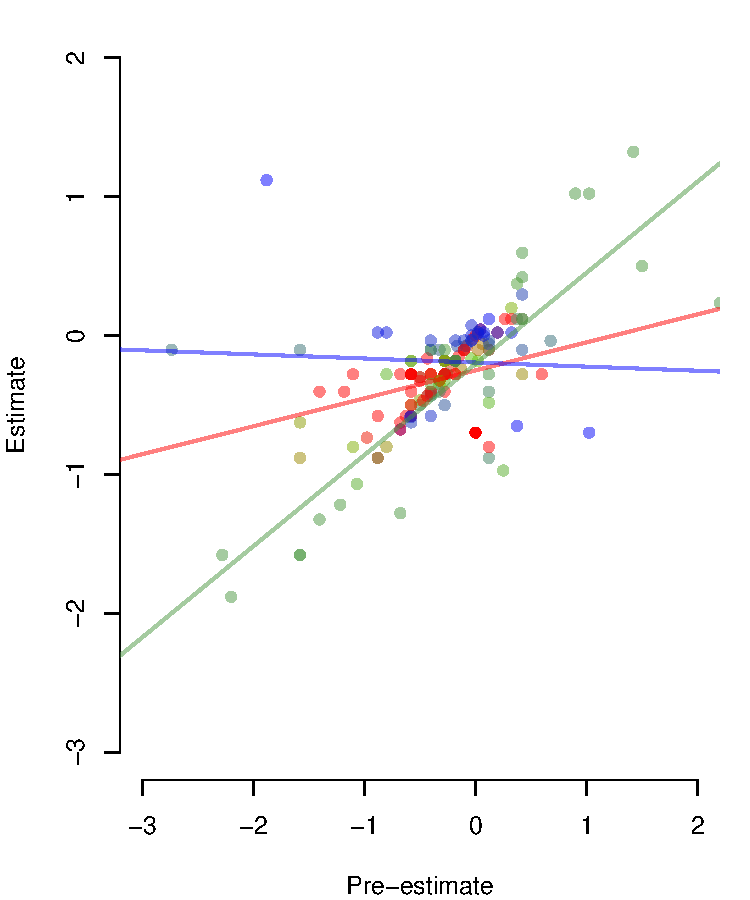
\includegraphics[width=\textwidth]{../plots/jayles1_vs_xp.pdf}
		\caption{Jayles question 1}
	\end{subfigure}
	\begin{subfigure}[b]{.24\textwidth}
		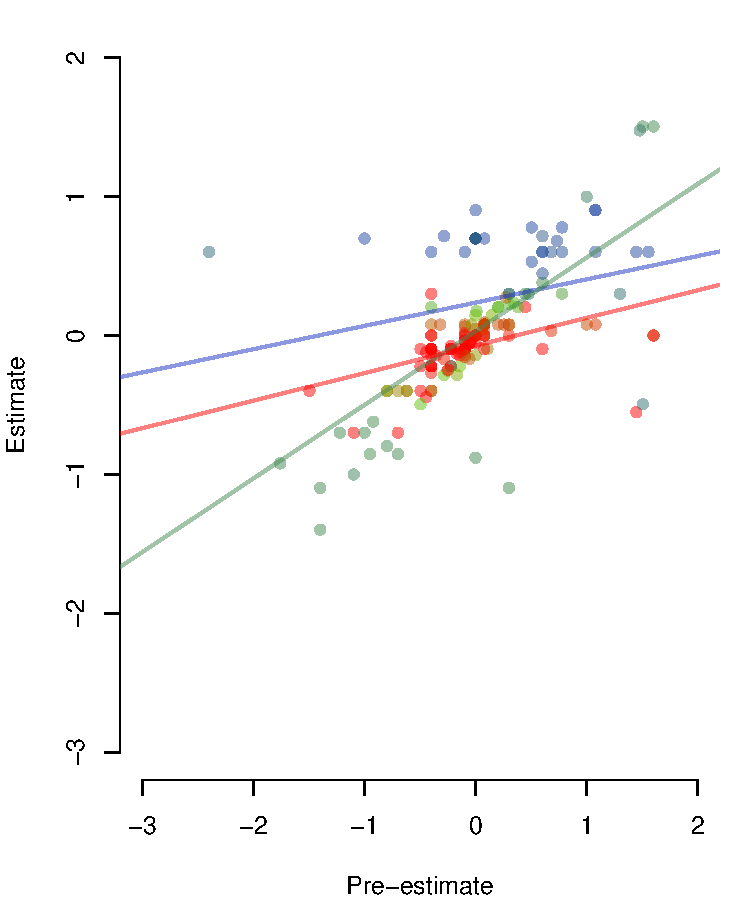
\includegraphics[width=\textwidth]{../plots/jayles2_vs_xp.pdf}
		\caption{Jayles question 2}
	\end{subfigure}
		\begin{subfigure}[b]{.24\textwidth}
		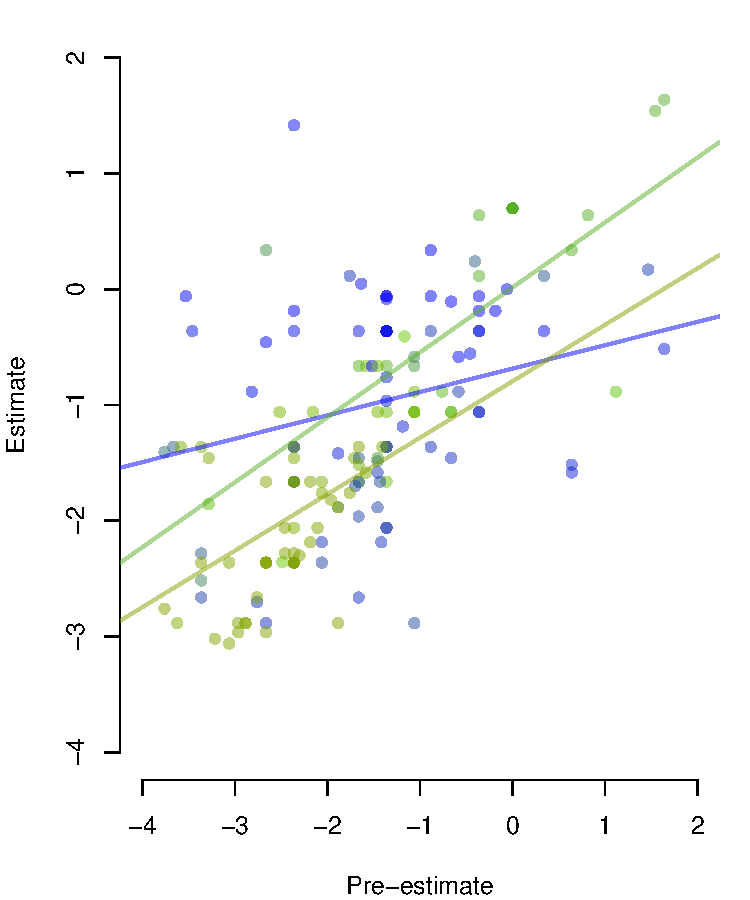
\includegraphics[width=\textwidth]{../plots/jayles8_vs_xp.pdf}
		\caption{Jayles question 8}
	\end{subfigure}
	\begin{subfigure}[b]{.24\textwidth}
		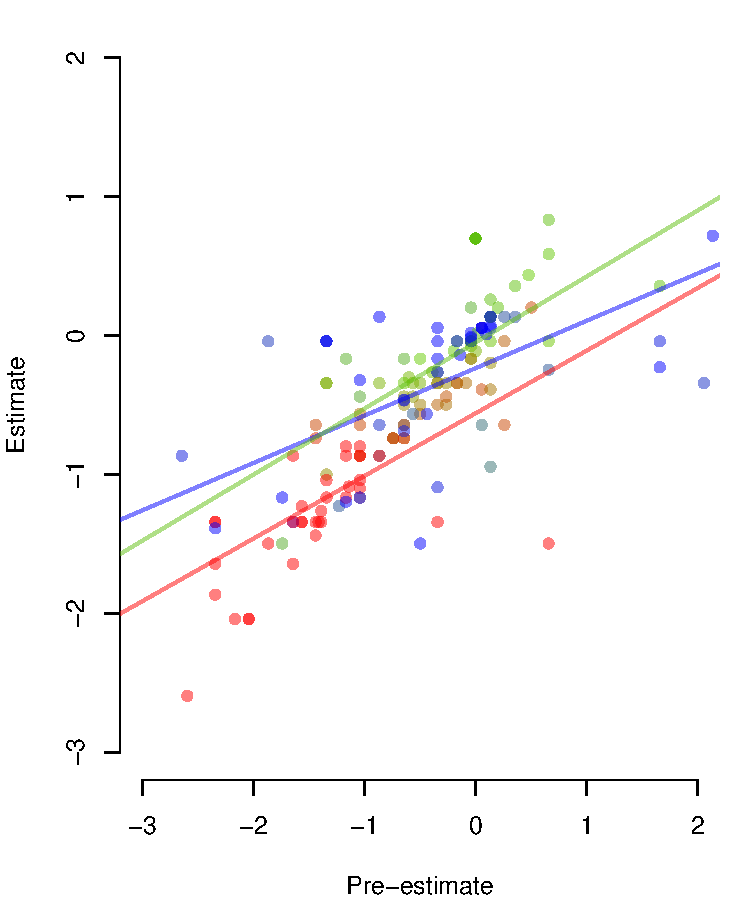
\includegraphics[width=\textwidth]{../plots/jayles10_vs_xp.pdf}
		\caption{Jayles question 10}
	\end{subfigure}
	\begin{subfigure}[b]{.24\textwidth}
		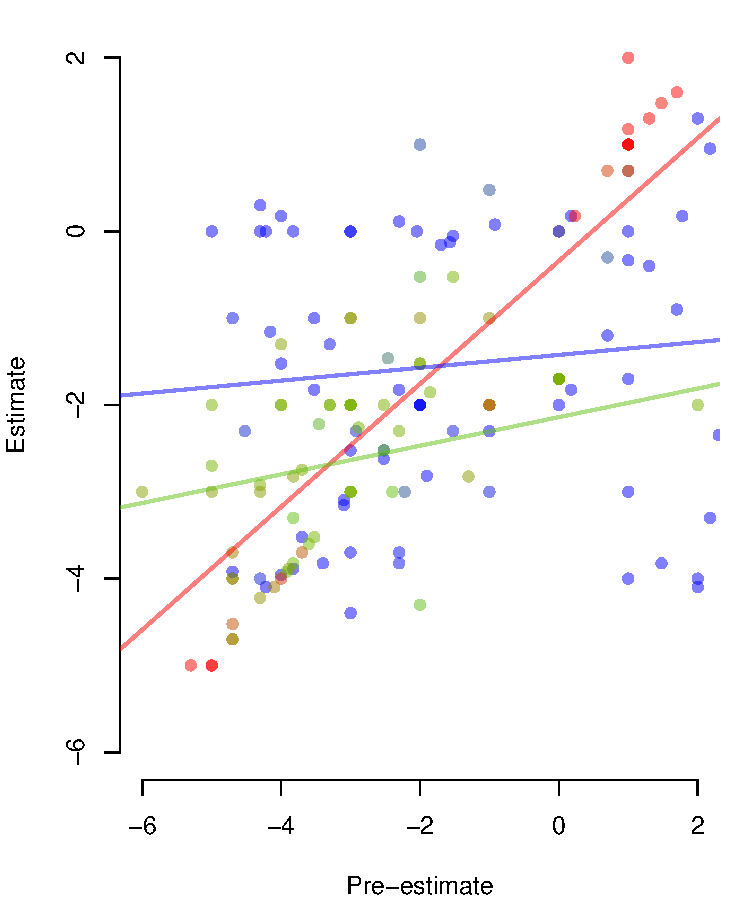
\includegraphics[width=\textwidth]{../plots/jayles23_vs_xp.pdf}
		\caption{Jayles question 23}
	\end{subfigure}
	\caption{Pre-estimates $y_i^0$ against final estimates $y_i$, with weighted regression lines. Colors are identical to the previous figures, and refer to the $\beta_w$ estimate. The regression lines are colored according to the same scheme, using their estimates slopes.}\label{fig: Jayles estimate vs pre-estimate}
\end{figure}

"Sed ut perspiciatis unde omnis iste natus error sit voluptatem accusantium doloremque laudantium, totam rem aperiam, eaque ipsa quae ab illo inventore veritatis et quasi architecto beatae vitae dicta sunt explicabo. Nemo enim ipsam voluptatem quia voluptas sit aspernatur aut odit aut fugit, sed quia consequuntur magni dolores eos qui ratione voluptatem sequi nesciunt. Neque porro quisquam est, qui dolorem ipsum quia dolor sit amet, consectetur, adipisci velit, sed quia non numquam eius modi tempora incidunt ut labore et dolore magnam aliquam quaerat voluptatem. Ut enim ad minima veniam, quis nostrum exercitationem ullam corporis suscipit laboriosam, nisi ut aliquid ex ea commodi consequatur? Quis autem vel eum iure reprehenderit qui in ea voluptate velit esse quam nihil molestiae consequatur, vel illum qui dolorem eum fugiat quo voluptas nulla pariatur?"
"Sed ut perspiciatis unde omnis iste natus error sit voluptatem accusantium doloremque laudantium, totam rem aperiam, eaque ipsa quae ab illo inventore veritatis et quasi architecto beatae vitae dicta sunt explicabo. Nemo enim ipsam voluptatem quia voluptas sit aspernatur aut odit aut fugit, sed quia consequuntur magni dolores eos qui ratione voluptatem sequi nesciunt. Neque porro quisquam est, qui dolorem ipsum quia dolor sit amet, consectetur, adipisci velit, sed quia non numquam eius modi tempora incidunt ut labore et dolore magnam aliquam quaerat voluptatem. Ut enim ad minima veniam, quis nostrum exercitationem ullam corporis suscipit laboriosam, nisi ut aliquid ex ea commodi consequatur? Quis autem vel eum iure reprehenderit qui in ea voluptate velit esse quam nihil molestiae consequatur, vel illum qui dolorem eum fugiat quo voluptas nulla pariatur?"

\begin{figure}[htbp]
	\centering
	\begin{subfigure}[b]{.24\textwidth}
		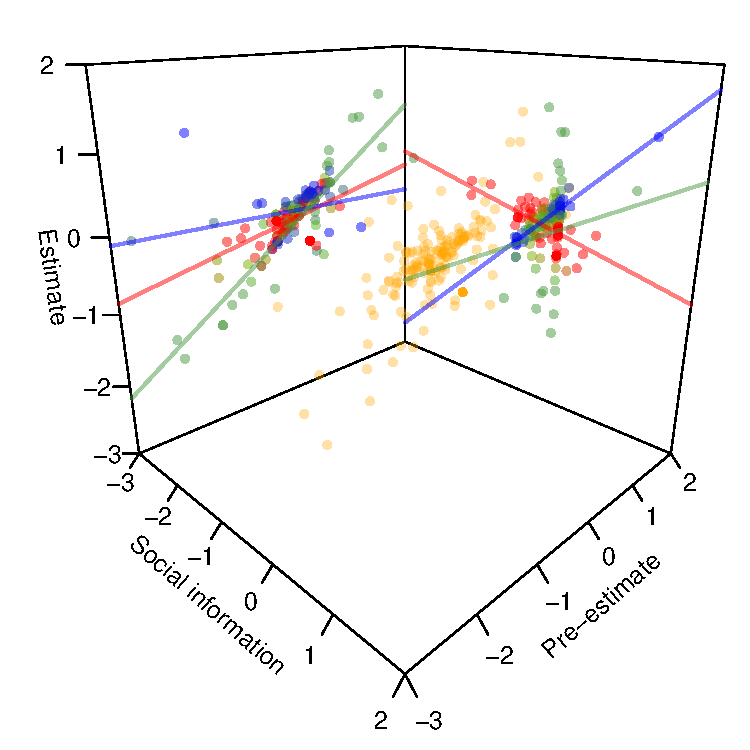
\includegraphics[width=\textwidth]{../plots/jayles1_vs_xp3d.pdf}
		\caption{Jayles question 1}
	\end{subfigure}
	\begin{subfigure}[b]{.24\textwidth}
		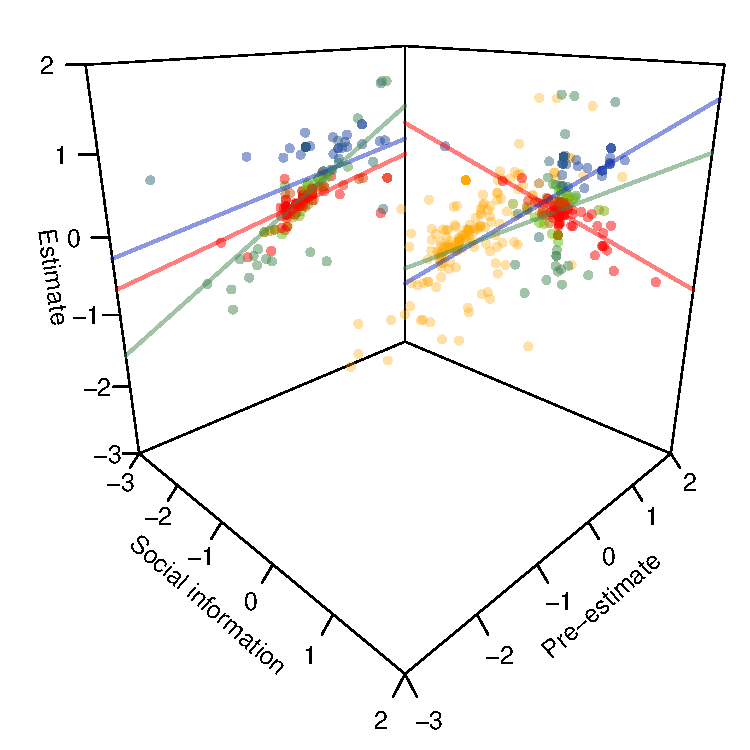
\includegraphics[width=\textwidth]{../plots/jayles2_vs_xp3d.pdf}
		\caption{Jayles question 2}
	\end{subfigure}
		\begin{subfigure}[b]{.24\textwidth}
		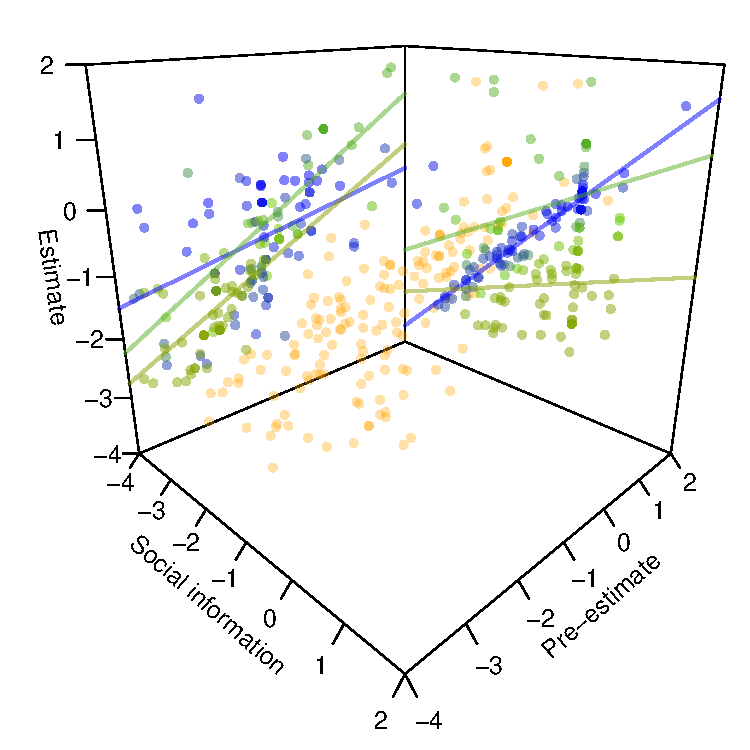
\includegraphics[width=\textwidth]{../plots/jayles8_vs_xp3d.pdf}
		\caption{Jayles question 8}
	\end{subfigure}
	\begin{subfigure}[b]{.24\textwidth}
		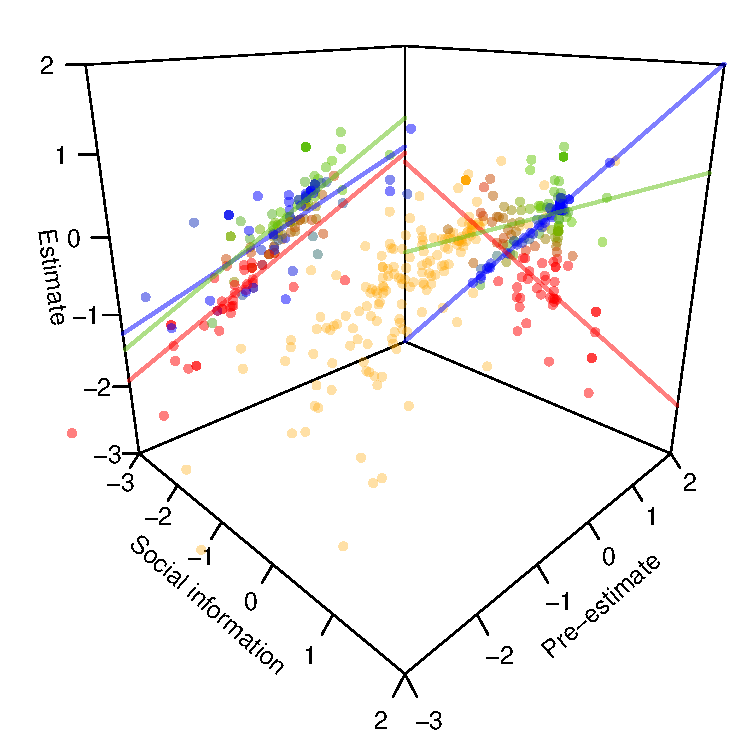
\includegraphics[width=\textwidth]{../plots/jayles10_vs_xp3d.pdf}
		\caption{Jayles question 10}
	\end{subfigure}
	\begin{subfigure}[b]{.24\textwidth}
		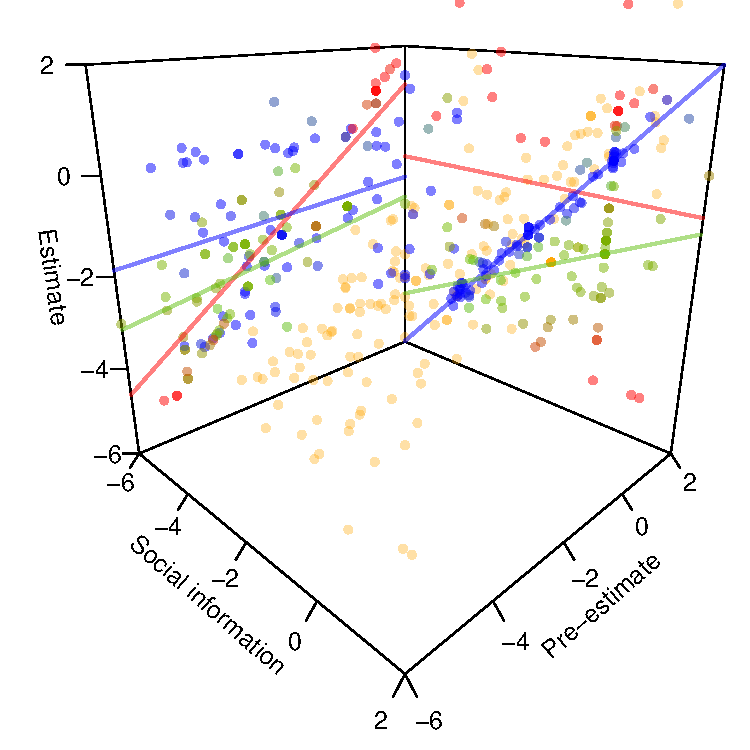
\includegraphics[width=\textwidth]{../plots/jayles23_vs_xp3d.pdf}
		\caption{Jayles question 23}
	\end{subfigure}
	\caption{Pre-estimates $y_i^0$ against final estimates $y_i$ and social information $m_i$, with weighted regression lines. Colors are identical to the previous figures, and refer to the $\beta_w$ estimate. The regression lines are colored according to the same scheme, using their estimates slopes.}\label{fig: Jayles 3d}
\end{figure}

















%%% Each figure should be on its own page
\begin{figure}
\centering
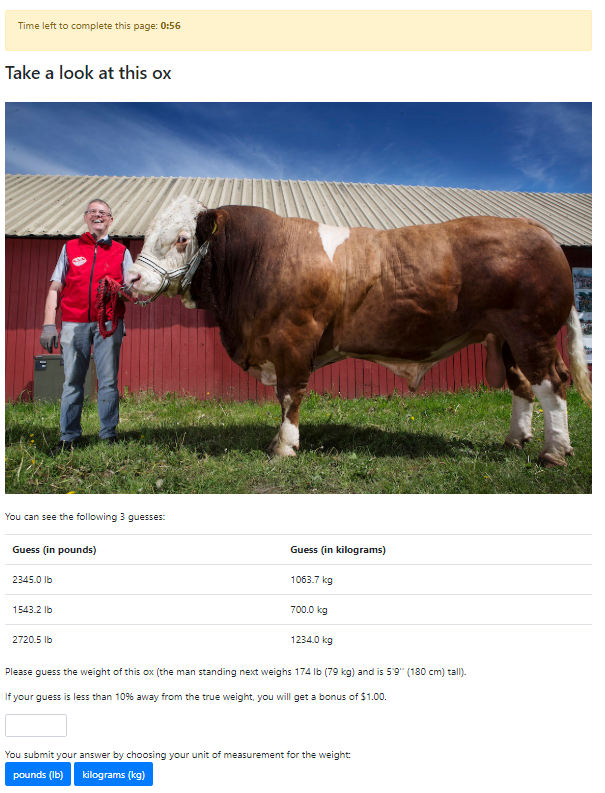
\includegraphics[width=.8\textwidth]{C:/Users/hjl161/Documents/Papers/WoT_github/images/FigS1.png}
\caption{Screendump of the choice-page in the ox-experiments with $v=3$. On image: The ox Hansi and his owner Mogens. Photo Credits: Klaus Holsting.}
\end{figure}

\begin{figure}
\centering
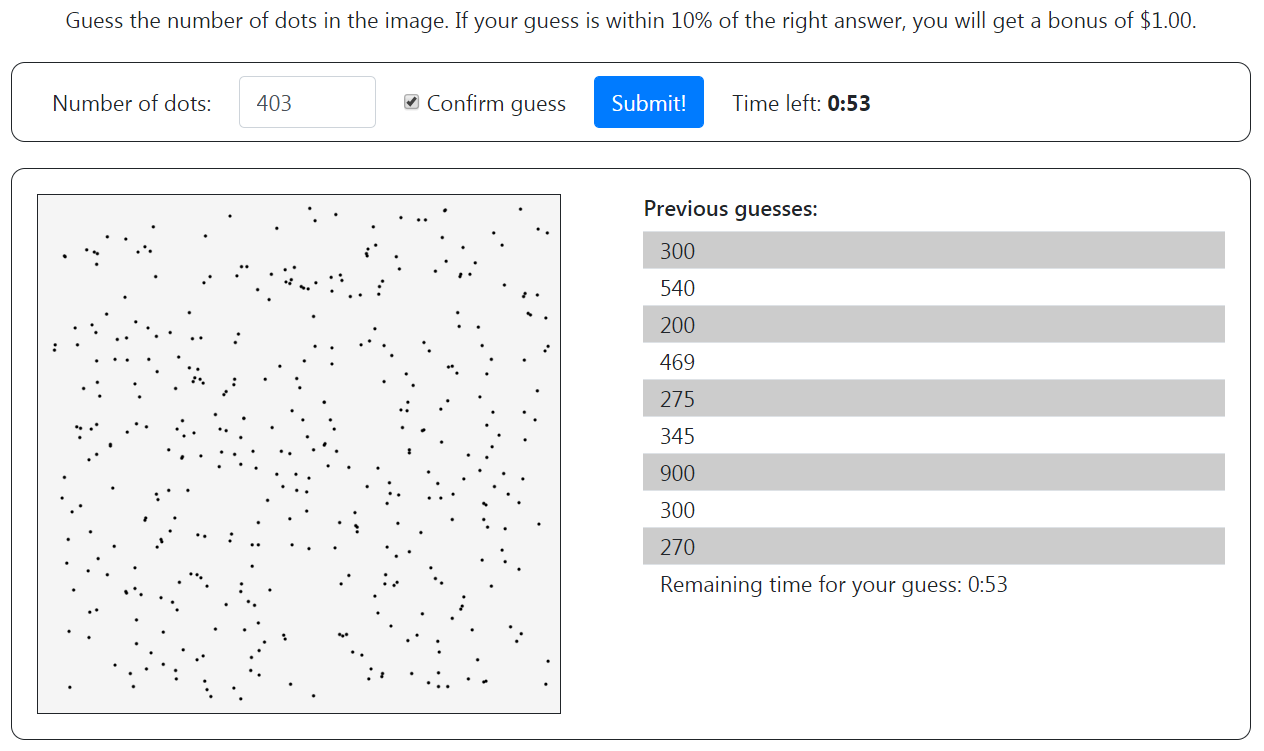
\includegraphics[width=.8\textwidth]{C:/Users/hjl161/Documents/Papers/WoT_github/images/FigS2.png}
\caption{Screendump of the choice-page in the dot-experiment with $d=403$ and $v=9$.}
\end{figure}


\begin{figure}
	\begin{subfigure}[b]{.8\textwidth}
		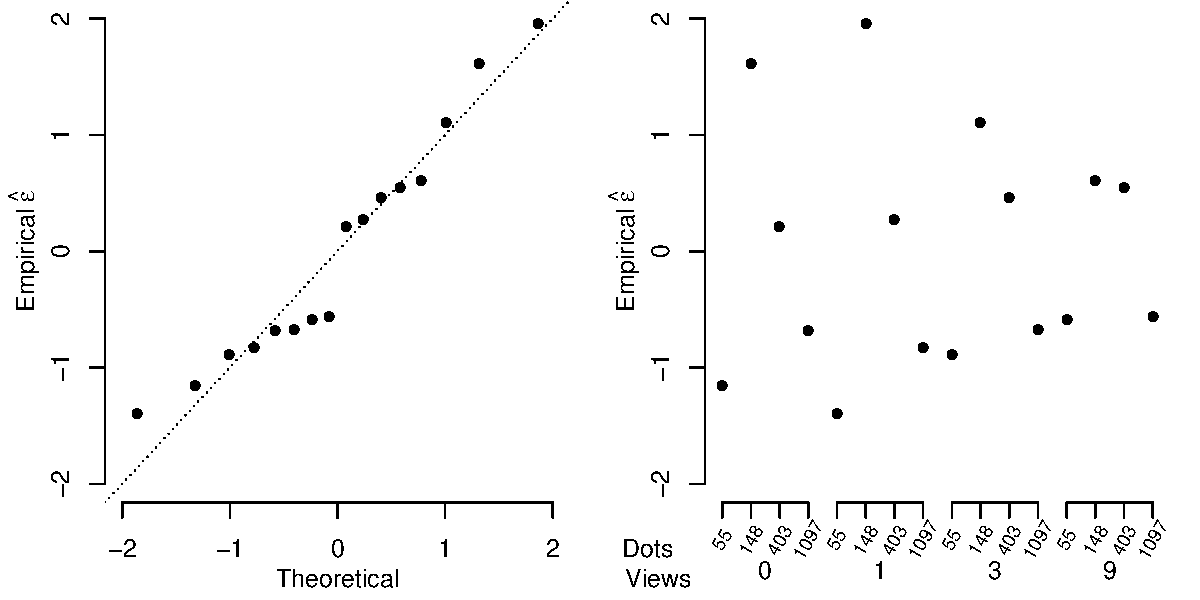
\includegraphics[width=\textwidth]{../plots/med_residual_h.pdf}
	\end{subfigure}
	\begin{subfigure}[b]{.8\textwidth}
		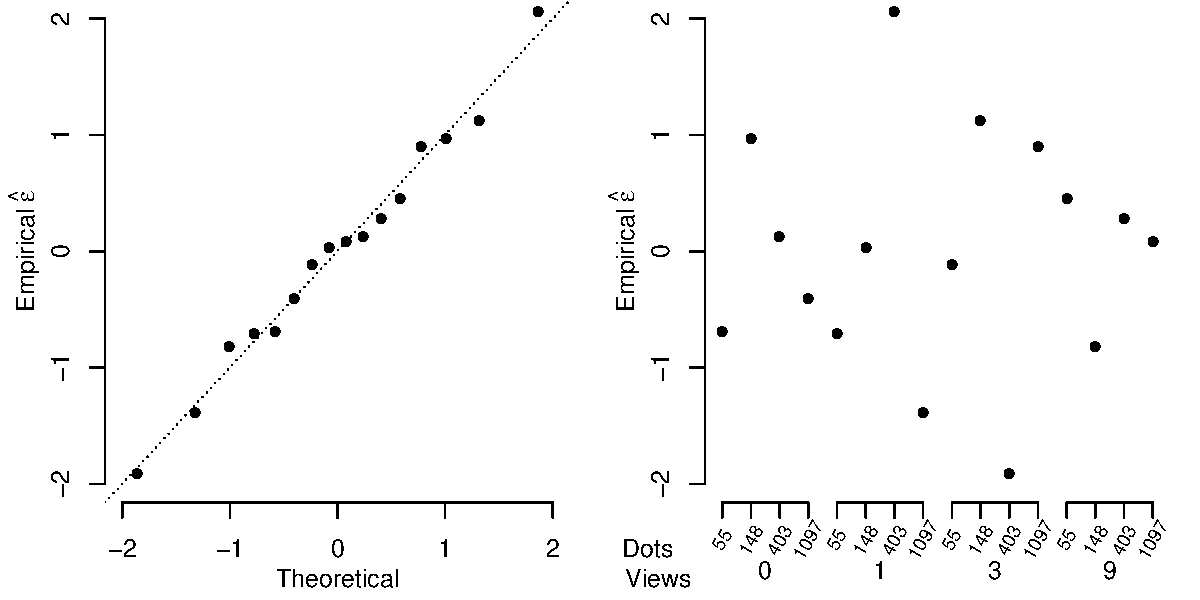
\includegraphics[width=\textwidth]{../plots/med_residual_m.pdf}	
	\end{subfigure}
	\caption{QQ plots for median analysis}
	\label{fig: qq plots median}
\end{figure}


\begin{sidewaysfigure}
	\centering
	\hfill
	\includegraphics[width=1\linewidth]{../plots/qqplots_AMT.pdf}			
	\caption{QQ plots for all threads}
	\label{fig: qq plots Mturk data}
	\hfill
\end{sidewaysfigure}


\begin{figure}
	\centering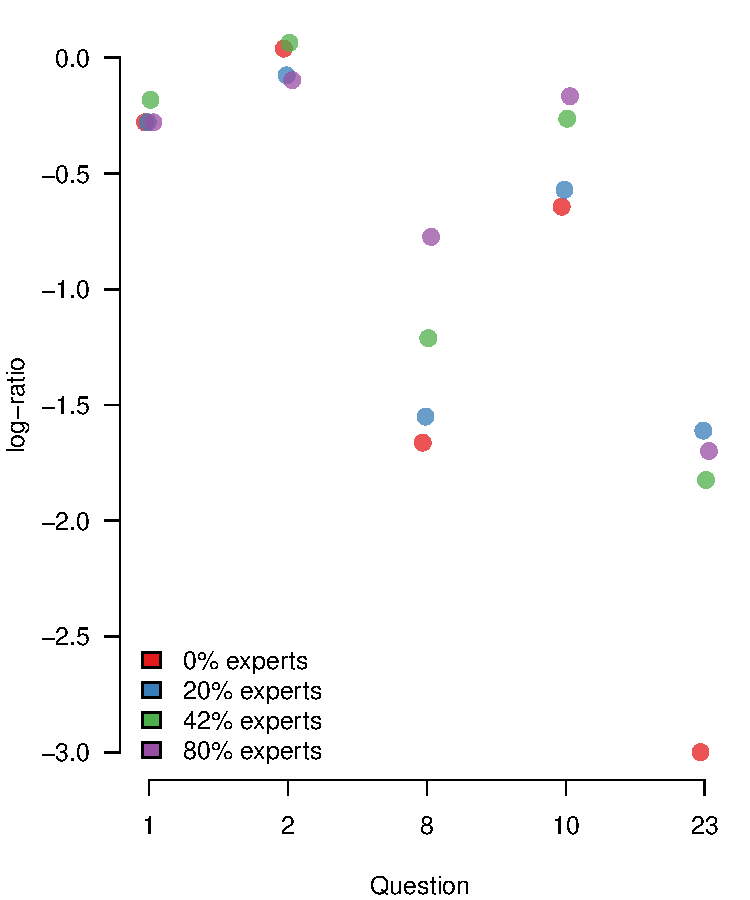
\includegraphics[width=.7\textwidth]{../plots/jayles_difficulty.pdf}
	\caption{Difficulty of Jayles questions 1, 2, 8, 10 and 23 as evaluated by the log-ratio of the group median.}
	\label{fig: Jayles question difficulty}
\end{figure}









\begin{table}\centering
\caption{Data Table of all threads. Legend: $d \in \{55, 148, 403, 1097\}$; $v$ = view count; method: \'history\'-threads show the preceding estimates as they have been recorded in the thread; N = thread length; median = median of thread; mean = mean of thread; SD = standard deviation; CV = coefficient of variation; skew = skewness; kurt = kurtosis; bonus = percentage of estimates within 10 \% of the true value, $d$.}

\begin{tabular}{lrrlrrrrrrrr}
\hline
 method   &    d &   v & thread   &   N &   median &     mean &       SD &    CV &   skew &   kurt &   bonus (\%) \\
\hline
 history  &   55 &   0 & fscmakcz & 464 &     55   &  2360.57 & 42038.6  & 17.81 &  21.01 & 445.08 &        60.13 \\
 history  &   55 &   1 & hs6bovtz & 477 &     57   &  1682.13 & 29381.7  & 17.47 &  21.18 & 453.74 &        55.35 \\
 history  &   55 &   3 & 3cda8qpn & 405 &     56   &  8320.59 & 73524.4  &  8.84 &   9.59 &  93.58 &        62.47 \\
 history  &   55 &   9 & bvpj37io & 476 &     56   &  1239.85 & 25435.5  & 20.51 &  21.74 & 470.87 &        54.83 \\
 history  &  148 &   0 & dwnjf9mb & 464 &    140   &  1349.14 & 12891    &  9.55 &  12.83 & 172.18 &        21.34 \\
 history  &  148 &   1 & ehaxc7lu & 435 &    150   &  2250.86 & 27802.5  & 12.35 &  15.66 & 261.32 &        24.83 \\
 history  &  148 &   3 & ck291lk5 & 466 &    147.5 &  2523.51 & 38071.3  & 15.09 &  20.42 & 427.38 &        22.53 \\
 history  &  148 &   9 & 2hxe3g0w & 473 &    153   &  3182.51 & 38085.7  & 11.97 &  13.85 & 196.79 &        24.1  \\
 history  &  403 &   0 & hqx0v7t5 & 473 &    300   &  4816.02 & 49624.9  & 10.3  &  14.16 & 220.03 &         7.82 \\
 history  &  403 &   1 & 9bbkjlye & 469 &    320   &  2791.59 & 31667.6  & 11.34 &  15.23 & 248.43 &         7.89 \\
 history  &  403 &   3 & 5du4txa7 & 455 &    350   &  2430    & 29944.3  & 12.32 &  15.25 & 233.19 &        11.21 \\
 history  &  403 &   9 & spw8qdcd & 470 &    400   &  3035.65 & 36078.8  & 11.89 &  15.32 & 235.27 &        10.21 \\
 history  & 1097 &   0 & hal5jdl0 & 423 &    657   &  8855.13 & 76379.1  &  8.63 &  11.46 & 138.21 &         9.69 \\
 history  & 1097 &   1 & z0rvh02v & 473 &    650   &  8091.24 & 68728.9  &  8.49 &  11.74 & 144.62 &         8.67 \\
 history  & 1097 &   1 & huyygtho & 461 &    750   &  2924.95 & 25012.2  &  8.55 &  17.91 & 344.84 &         9.11 \\
 history  & 1097 &   3 & hhb0if6e & 470 &    812.5 &  4811.97 & 53329.9  & 11.08 &  15.61 & 259.91 &        20.43 \\
 history  & 1097 &   9 & wv4xujg7 & 460 &    999   &  2748    & 31206.8  & 11.36 &  21.24 & 451.09 &        13.48 \\
 max      &   55 &   1 & aebicytb & 384 &     57   &    68.7  &    35.77 &  0.52 &   2.82 &   8.76 &        51.04 \\
 max      &   55 &   3 & 094p61xp & 340 &     60   &   101.05 &   413.25 &  4.09 &  18    & 326.23 &        41.18 \\
 max      &   55 &   9 & 8c80yyxl & 418 &     60   &    75.03 &    45.69 &  0.61 &   4.72 &  34.23 &        50.72 \\
 max      &  148 &   1 & 78wuly7l & 317 &    152   &   271.06 &   323.75 &  1.19 &   3.84 &  19.06 &        14.51 \\
 max      &  148 &   3 & u2sxnl2p & 418 &    220   &   366.6  &   596    &  1.63 &  11.6  & 179.79 &         9.57 \\
 max      &  148 &   9 & mf57hnwb & 412 &    210   &   266.74 &   168.39 &  0.63 &   1.08 &   0.2  &        11.89 \\
 max      &  403 &   1 & 6c4s02ki &  16 &     90   &   452.5  &   614.18 &  1.36 &   2.26 &   4.85 &         0    \\
 max      &  403 &   1 & 1r17post &  25 &    400   &   549    &   402.64 &  0.73 &   1.83 &   4.14 &         4    \\
 max      &  403 &   1 & e8vv9575 &  64 &    600   &   734.38 &   506.71 &  0.69 &   0.48 &  -1    &         6.25 \\
 max      &  403 &   3 & ua2230ux & 315 &    600   &  3215.08 &  9635.18 &  3    &   4.84 &  22.79 &         7.94 \\
 max      &  403 &   9 & 1xyev3dj & 422 &    887.5 &  4758.88 & 25397.5  &  5.34 &  17.68 & 339.78 &         7.82 \\
 max      & 1097 &   1 & 7yqp8bxc & 116 &    800   &  5463.93 & 15517.2  &  2.84 &   4.21 &  16.95 &         8.62 \\
 max      & 1097 &   1 & q5brhgnz &  76 &   1062.5 &  3310.3  &  4690.72 &  1.42 &   2.13 &   4.19 &         5.26 \\
 max      & 1097 &   3 & 2x6km84z & 117 &   2500   &  7593.38 &  9341.25 &  1.23 &   1.29 &   0.35 &        13.68 \\
 max      & 1097 &   3 & ud5vo371 &  78 &   2950   &  5167.06 & 12588.5  &  2.44 &   7.43 &  58.71 &         2.56 \\
 max      & 1097 &   9 & lh7wb36v & 416 &   3410   & 13024.2  & 38664.1  &  2.97 &  11.9  & 183.47 &         7.93 \\
\hline
 &&&& 11.748 &&&&&&& \\
\bottomrule
\end{tabular}



\end{table}\label{table:S1}

%%% Add this line AFTER all your figures and tables
\FloatBarrier

\dataset{dots.csv}{Anonymized data set of all dots-experiments. Parameters: task = type of experiment; d = number of dots in image; v = number of visible preceding estimates; session = thread name; code = unique identifier of participant; id = participant id in thread; order = order in which participants enter the queue; hist = list of preceding id's having made an estimate; guess = estimate by participant; bonus = payoff in dollars if estimate was within 10\% of d.}

\dataset{ox.csv}{Anonymized data set of all ox-experiments. Parameters: task = type of experiment; d = weight of the ox (in kilo); v = number of visible preceding estimates; session = thread name; code = unique identifier of participant; id = participant id in thread; order = order in which participants enter the queue; hist = list of preceding id's having made an estimate; guess = estimate by participant; pound = 1 if estimate was made in lb, 0 if estimate was made in kg; bonus = payoff in dollars if estimate was within 10\% of d.}

\bibliography{wamot}
%\bibliographystyle{naturemag}

\end{document}